\section{Koord Software Stack}
\label{sec:software}

\subsection{Runtime system}



To run a $\lgname$ program (hardware or simulation), the user has to provide a configuration file, with 
\begin{inparaenum}
\item the number of agents, 
\item in case of simulation, the initial positions of the agents and the length of the simulation and 
\item in case of hardware deployment their IP addresses, 
and the localization system.
\end{inparaenum} 

\subsection{Key environment assumptions} 


\subsubsection{Periodic event execution semantics}


\subsubsection{Shared variable implementation over message passing}


\subsubsection{Known set of participants}
\subsubsection{Portability and heterogeneity}


\subsection{Simulator}
\subsubsection{gazebo environment}
\subsubsection{car model}
\subsubsection{lidar}
\subsubsection{positioning}
\subsubsection{sampled sensing}
\subsubsection{synchronization issues}
 
\subsection{The Distributed Mapping Problem}
In this section, we introduce the distributed mapping problem that the $\lgname$ program shown in \reffig{mapapp} aims to solve. The key difference between distributed SLAM and this application is that we assume that the robots know their \emph{global coordinates} within the area of deployment. They are only attempting to map the static obstacles within this area.

Informally, the problem requires a set of robots to collaboratively agree on positioning of static \emph{obstacles} within a given area $D$, which any robot should avoid while moving in $D$. We currently assume that the only sensors available for sensing obstacles are LIDAR based, and the robots are constrained to move in a 2-D space.


\subsubsection{Preliminaries}
\label{sec:prelims}
We first set up the terminology and assumptions to discuss our approach to this problem. 

The mapping problem is defined over a (\emph{bounded}) domain $D$. In our problem setup, we assume $D$ is a rectangle in $\mathbb{R}^2$ given by $[x_1,x_2]\times [y_1,y_2]$.

\begin{definition}
A \emph{quantization} of a bounded domain $D$ is defined as a mapping $\qfunc:D \mapsto \qdom$, where $\qdom$ is a discrete set. If $\qdom$ is, for instance, $\mathbb{Z}\times \mathbb{Z}$, this can be viewed as an embedding of a 2D-lattice in $\mathbb{R}^2$. 
\end{definition}

In theory, we can assume the existence of a \emph{ground truth} function $\world : D\mapsto \left\{0,1\right\}$, where $$\world(\Vec{x}) = \begin{cases}
1\ \mbox{if there is an obstacle at }\Vec{x}\\
0\ \mbox{otherwise}
\end{cases}
$$

Given any quantization $Q$ of the domain $D$ given by $\qfunc:D\mapsto Q$, the corresponding \emph{quantized} ground truth function 
$\world_Q : Q \mapsto \left\{0,1\right\}$ is defined as follows,  $$\world_Q(q) = \begin{cases}
1\ \Leftrightarrow \exists \Vec{x}\in D, \qfunc(\Vec{x}) = q \wedge \world(\Vec{x}) = 1 \\
0\ \mbox{otherwise}
\end{cases}
$$
\rg{Consider that there is a set of ground robots $[N]$, which are tasked with creating a mapping of static obstacles in $Q$ collaboratively by constructing local mappings based on sensed information.}

Let $\map_i:Q\mapsto \left\{-1,0,1\right\}$ denote a construction of a map function \emph{local} to robot $i$, where, $\map_i(q) = 1$ indicates that according to robot $i$, there is an obstacle in $q$, $\map_i(q) = 0$ indicates that according to robot $i$, $q$ is unoccupied, and $\map_i(q) = -1$ indicates that robot $i$ doesn't have information about $q$. 

\begin{definition} The \emph{sensing area} of a robot $i$ at position $\pos(i)$ is defined by $\sensarea: Q \mapsto 2^{Q}$, such that $\map_i(\sensarea(\qfunc(pos(i))) = \world_Q(\sensarea(\qfunc(pos(i))$.  
  \end{definition}


We can then state the 2-d distributed mapping problem, $\mapprob$ as follows. \begin{quote}
 {\em Given a quantization, $\qfunc:D\mapsto Q$ of a 2-d domain $D\subset \mathbb{R}^2$, a ground truth function $\world:D \mapsto \left\{0,1\right\}$, a set of robots $[N]$ , for each robot $i \in [N]$ construct an occupancy mapping, $\map_i: Q \mapsto \left\{1,0,-1\right\}$, such that $\forall i , j \in [N], \forall q \in Q, \forall v \in \left\{0,1\right\}$:
$$ (map_i(q) = v \Rightarrow
 map_j(q) = v \vee map_j(q) = -1)$$
 }
\end{quote}

 \rg{We can then \emph{combine} the elements of the set of \emph{local maps}, $\{\map_i\}_{i\in [N]}$ to form a \emph{global} occupancy mapping, $\map: Q\mapsto \left\{-1,0,1\right\}$ where $\map(q) = Max(\{\map_i(q)\}_{i\in[N]})$.}
 
A vacuously correct solution to $\mapprob$ given $D, \qfunc$ and $\world_Q$ is $\forall i \in [N]$, $$\map_i : Q \mapsto \left\{0,1,-1\right\}, \forall  q \in Q , \map_i(q)= -1$$ To allow for other solutions than the one stated above, we assume that we are given that initially, each robot $i\in[N]$ starts at a grid square with no obstacle, and the occupancy function $\map_i$ is initialized as follows:
 $\forall i \in [N], \world_Q(\qfunc(\mathit{ipos}(i))) = 0$ and 
 $\forall i \in [N], \map_i(\qfunc(\mathit{ipos}(i))) = 0$,
  where $\mathit{ipos}(i)$ denotes the initial position of the robot $i$. 

Having stated the problem, we now define the notion of soundness of a proposed occupancy map w.r.t an instance of $\mapprob$. 
\begin{definition}
\label{soundness}
Given an instance of $\mapprob$ with domain $D$, a quantization $\qfunc: D\mapsto Q$, ground truth mapping $\world:D \mapsto \left\{0,1\right\}$, a proposed occupancy mapping, $\map: Q \mapsto \left\{-1,0,1\right\}$ is \emph{sound} if :
\begin{itemize}
\item $\forall v \in \left\{0,1\right\} \map(q) = v \Rightarrow \world_Q(q)  = v$
\item $\forall v \in \left\{0,1\right\}\world_Q(q) = v \Rightarrow \map(q) = v \vee \map(q) = -1$
\end{itemize}
\end{definition}

These two statements collectively state that given a proposed occupancy map, \emph{any grid point marked as 0 is indeed obstacle free, and if it is marked as 1 then there is indeed an obstacle at least partially in it.}  An algorithm for $\mapprob$ is \emph{sound} if its output occupancy map is sound according to \defn{soundness}.

We assume that at time $t$, if robot $i$ detects an obstacle in $q \in \sensarea(\qfunc(\pos_t(i)))$ , then $q$ does contain an obstacle, otherwise it does not. The point of this presentation isn't dealing with the issue of potentially false positives while identifying an obstacle. A robot partially constructs a grid occupancy function by assigning values to the grid squares in its \emph{sensed} area.





\subsubsection{Approach}
We discuss now discuss how our algorithm implemented $\lgname$ shown in \reffig{mapapp} tackles $\mapprob$. \reffig{flowmap} shows each agent's approach towards solving $\mapprob$. 

\begin{figure}[!htbp]
    \centering
    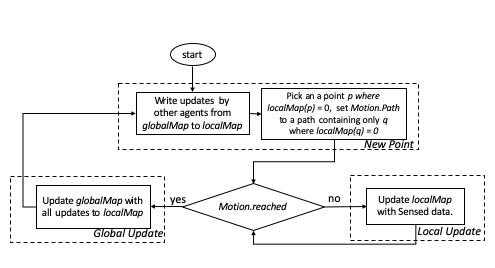
\includegraphics[width=\linewidth]{figs/map_flowchart.png}
    \caption{Flowchart for a simple solution to 2D distributed mapping problem\vspace{-2mm}}
    \label{fig:flowmap}
\end{figure}

The variable $\lmap$ refers to each agent's current \emph{view} of $\map$ being constructed by the algorithm. The function $\mathit{MaxExp}$ informally, determines whether the maximum exploration of the map required by the algorithm (in the agent's view) has been completed. If not, the agent first updates its $\lmap$ from $\gmap$, which contains the map of obstacles and unoccupied squares created collaboratively from $\lmap$s of all agents so far. The agent then picks a new point in a square known to be unoccupied in its $\lmap$ and sets $\mathit{Motion.Path}$ to a path moving only over squares known to be unoccupied by its $\lmap$. While the agent hasn't reached the target square, it keeps updating its $\lmap$ with sensed data (occupied and unoccupied squares). When it reaches the target square, it updates the $\gmap$ with its $\lmap$ information, letting all other agents know the map discovered by it. In terms of our formalization presented in \refsect{prelims}, the final value of $\gmap$ corresponds to the constructed grid occupancy mapping, $\map$. 






\begin{theorem}
The $\lgname$ application shown in \reffig{mapapp} implements a sound algorithm for any input instance of $\mapprob$.
\end{theorem}

\subsubsection{External (Library) Functions}

